\chapter[Short Chap title]{This chapter has a very long title that would be too long for using in headers and table of contents}
\section{Image processing}
Because Image processing is such a large topic no attempt will be made
here to describe the entire subject here but only areas directly
relevant to the project as a whole. Note how we can cross reference
sections of the document such as section~\ref{pg:filters}

\section{Low level operations}
\label{pg:filters}
Here is an example of a list with bullets:
\begin{itemize}
\item{\it Mean} Take the mean value of the neighbourhood.

\item{\it Median Filter} Take the median value of the neighbourhood.
\end{itemize}

Here are a couple of mathematical formulae:
\begin{quote}
\centering
$\Delta_1=I(x,y)-I(x+1,y+1)$ \\
$(x-a)^2+(y-b)^2=R^2$
\end{quote}

A table is just like a figure. Table~\ref{wombat} uses the tabular
environment.  Environments such as tabular can be used in ordinary
text as well.
\begin{table}
\begin{center}
\begin{tabular}{|r|c|c|c|}\hline\hline
place&1991&1992&1993\\\hline
CS Dept& 1&99&199\\
Owens Park& 1876& 22&0\\
Academy&0&0&99999\\\hline\hline
\end{tabular}
\end{center}
\caption{Distribution of Wombats in Greater Manchester}\label{wombat}
\end{table}


\section{Creating Diagrams}
\label{sec:diagrams}

Figure~\ref{fig:fig-eg} is a figure previously prepared using the
\texttt{xfig} interactive drawing package. With the latest version of
\texttt{xfig} it is quite easy to incorporate \texttt{xfig} diagrams.
The \texttt{xfig} package is menu driven and reasonably self
explanatory.

Use the \emph{Export} menu option to save an encapsulated PostScript
version of your figure, which can then be included in the document
using the \verb=\includegraphics= command. Choose the \emph{Portrait}
orientation option. For example, if the figure is in the file \textsf{
  figure1.fig}, the exporting process will create a file \textsf{
  figure1.eps}, which can then be included, scaled to whatever height
or width you want.


\begin{figure}
\begin{center}
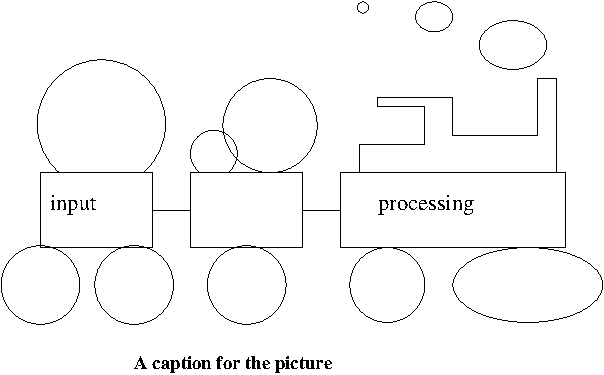
\includegraphics[width=10cm]{figure1} % This scales the picture to
                                      % a width of 10cm
                                      % You can scale to the
                                      % width or height you need
\end{center}
\caption{Final version of the system}
\label{fig:fig-eg}  
\end{figure}

Note that, if you want to use such graphics facilities in some other
document, which does not use either the \texttt{third-rep} or
\texttt{muthesis} document class, you will need to put the command
\verb=\usepackage{graphicx}= after the \verb=\documentclass....=
command in the main file.

\section{Screen Dumps}
\label{sec:screen-dumps}
\begin{figure}
\begin{center}
\includegraphics[width=12cm]{screen}
\end{center}
\caption{A screen dump}
\label{fig:scr-dump}
\end{figure}

Screen dumps can often enhance the appearance and clarity of a report,
although care should be taken not to overuse them. When using screen
dumps it is useful to make use of \LaTeX's capability for using
compressed PostScript files, as in the example shown in
figure~\ref{fig:scr-dump}. 

The image is first captured using, for example, \texttt{xv}, and saved
in a file, e.g.\ \texttt{screen.ps}. Next, extract the bounding box
information from the head of this file. In this case it is
\begin{verbatim}
%%BoundingBox: -100 -16 697 860
\end{verbatim}
and create a file with name given by adding \texttt{.bb} to the
original file name (in this case the name is \texttt{screen.ps.bb}) which
contains just this bounding box. You can now compress the original
file, using \texttt{gzip}. The command
\verb!\includegraphics[width=12cm]{screen}! will look for either
\textsf{screen.ps} or \textsf{screen.ps.gz}, so you can compress or
uncompress the \textsf{ps} file without changing the latex source.

Alternatively, save as \texttt{.png} if using \texttt{pdflatex}.

The \texttt{draft} option can be used to exclude the actual figure,
but leave an appropriate amount of space.

\textbf{You may not be able to see the screen dump if you are viewing this
file from WWW. This is due to an unfortunate `feature' of the
previewer xdvi.} If you view the files directly from
\texttt{/opt/info/doc/latex/3rd-yr}, things should work properly.

% Local Variables: 
% mode: latex
% TeX-master: "report"
% End: 
